\section{Implementation Mapping and Integration Boundaries}
\label{sec:implementation}

The implementation separates common protocol identities, model semantics,
backend physical work, and runtime coordination. CLI/HTTP interfaces deliver
caller-visible results; they are not the model driver's publication authority.
Table~\ref{tab:implementation-map} maps the preceding contracts to concrete
modules and names the coverage that must be checked before interpreting a run.
These are local implementation anchors, not a profile-wide correctness result.

\begin{table}[tbp]
\centering
\small
\begin{tabularx}{\linewidth}{@{}p{0.19\linewidth}>{\raggedright\arraybackslash}X>{\raggedright\arraybackslash}X@{}}
\toprule
Contract & Implementation anchor (under \texttt{crates/}) & Evaluation obligation \\
\midrule
Source-bound $P$ & \path{ferrule-model/src/checkpoint/}: catalog, source, read plan & Freeze source/representation; descriptor hash is not payload authentication \\
Exact $K,e$ & \path{ferrule-common/src/io_protocol.rs}: keys, completion, slabs, leases & Reject stale operation/stage/generation/byte evidence \\
Covered claims & \path{ferrule-runtime/src/scheduling/resources.rs}: \texttt{PhysicalResourceBroker} & Map ledgers to real allocations and final retained custody \\
Load publication & \path{ferrule-runtime/src/io/registry.rs}: reserve, completion, preflight, resident transfer & Verify provider transfer installs this registry on the evaluated path \\
Physical completion & \path{ferrule-model/src/moe/cuda_materialization.rs}: routed-expert provider & Trace pinned read, upload, install, replacement, and Unknown ownership \\
State publication & \path{ferrule-runtime/src/parallel/pipeline/owner.rs}; decoder KV and page manager & Journal before preparation; exact ACKs and retirement before reuse \\
\bottomrule
\end{tabularx}
\caption{Contract-to-code mapping. Common interfaces do not imply universal
registry integration or measured storage traffic.}
\label{tab:implementation-map}
\end{table}

\paragraph{Source binding and startup preparation.}
Checkpoint catalogs and read plans hold semantic tensor descriptors, ordered
file extents, and filesystem identity snapshots, not payload bytes. In this
adapter, \texttt{ContentHash} hashes dtype/shape/byte descriptors; source
identity additionally binds paths, offsets, and file metadata. Neither is a
read-and-hash authentication of every payload byte. The physical provider
resolves the plan against the residency authority and obtains the actual
destination generation. A startup CUDA image claim is a different authority
from a per-request load ticket: actual image grants, compiled context, image
fence, KV/initial-state creation, and the final claim fence are checked before
claim consumption. Eligible raw execution bindings may then be replaced by
runtime descriptors; surviving shared source aliases are not thereby freed.

\paragraph{General materialization path.}
The registry is installed only when a runner transfers a physical
materialization provider to the resident engine. It merges compatible exact
keys, validates completion before mutation, and separates return of stage
custody from credit release and resident-grant transfer. The concrete
routed-expert provider uses Linux pinned reads/io\_uring and CUDA upload/
installation. Registered slabs retain aligned ranges and exact generations;
upload tickets retain the original event and frame, even after notification
errors. Replacement passes the previous binding and old-consumer compute
proof to the install adapter. A generic lease completion contract is owner
metadata, not an independently recorded global GPU fence. Some preparation
helpers use compute and upload stream events; synchronization is not excluded.

The broker canonicalizes claims and validates their limits before charging.
Required execution can use a reserve unavailable to warmup/speculation, but
that does not guarantee progress if a provider stalls. Load admission is
stage-local, not an atomic reservation of all future stages. A later-stage
budget wait leaves earlier slabs/destinations charged. Returned provider
custody clears the submitted obligation, not occupancy; grants have no
implicit destructor refund. The five classes of
Equation~\ref{eq:credit-conservation} are therefore semantic refinements of
owner state, not five measured fields.

\paragraph{Owner-local state protocols.}
Ordinary TP1 pipeline segments use startup preparation, persistent stage
owners, and a prepared-KV journal; they do not automatically inherit registry
single-flight or I/O overlap. The provisional journal precedes backend
preparation because preparation can submit work before returning a handle.
Readiness validates existing evidence, not new submission. Lost install ACKs
poll the same identity without redispatch. Exact participant ACKs precede
logical publication, then displaced-state retirement and zero-reference-page
confirmation precede reuse. Finish consumes transaction-handle custody, not
live weights, KV, or independent pins. HostKV decode/idle reclaim use typed
read and placement/page-retirement protocols rather than the expert registry.
Committed-KV source snapshots include owner, slot, incarnation, generation,
layout, frontier, range, and pages; acquiring a read lease revalidates them,
and physical quiescence precedes pin release. Append witnesses are also
revalidated against the live reservation. These are not database snapshots.

\begin{figure}[tbp]
\centering
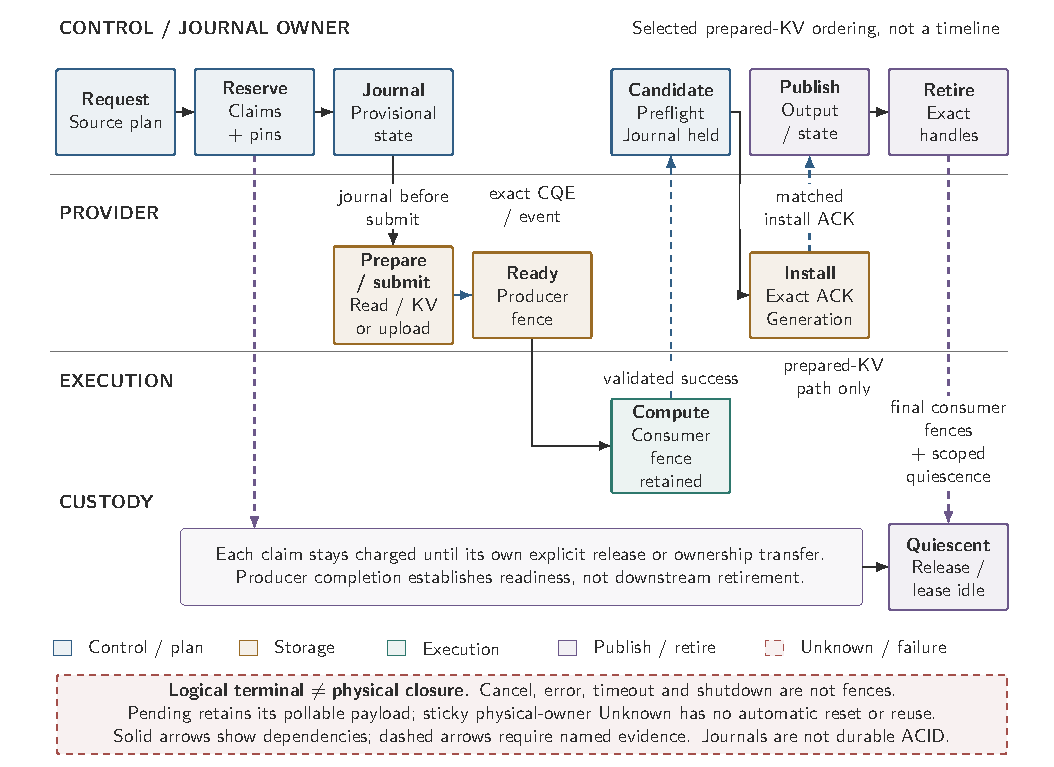
\includegraphics[width=\linewidth]{figures/transaction-lifecycle.pdf}
\caption{Conceptual successful lifecycle for the selected prepared-KV owner,
not a measured overlap timeline. Named lanes and swatches retain blue
control/validation, ochre materialization, teal execution, violet
publication/custody, and brick Unknown/failure roles. The provisional journal
precedes backend preparation even if submission fails without a handle.
Candidate readiness validates existing evidence; exact generation-matched
install ACKs precede logical publication on this path. Producer readiness is
not consumer retirement. Final relevant fences and scoped quiescence precede
custody return, with explicit release/transfer still required. Cancellation
cannot reverse irreversible ending. Neither durable ACID, universal registry
integration, nor general cross-rank atomicity follows.}
\label{fig:transaction-lifecycle}
\end{figure}

\paragraph{Unknown and collective scope.}
Provider Unknown retains native tickets, allocations, claims, and cleanup
intent, and may poison slot layers, devices, or executors. A matching registry
completion can close a named obligation without resetting independent poison.
There is no general in-place reset/replay or device-reset recovery claim.
Prepared-KV coordination is a narrow state lifecycle, not arbitrary distributed
atomic publication. Current collective exchanges have separate host-payload
bounds; Mixed device participation defaults to disabled/host. A typed device
permit is not evidence of a default GPU reduction or cross-rank fence. For the
vLLM supplement, Socket-plugin initialization is not proof that local GPU
payload used Socket: the scoped logs record \texttt{NCCL\_P2P\_DISABLE=1}
and local channels \texttt{via SHM/direct/direct}. No NCCL capability or
transport conclusion is generalized beyond the recorded profile.

\paragraph{What must be traced.}
A full path audit names each progress owner, queue/limit, dependencies,
submission behavior, completion evidence, blocking calls, locks, and
synchronization from request admission through storage, expansion, transfer,
execution, publication, retirement, cancellation, and shutdown. Include
model-specific and host-KV bypasses. A worker wrapping a blocking call is not
proof of event-driven progress or hardware overlap. Current BF16/numeric and
Mixed TP profiles have distinct shard/cache/expansion policies; actual storage
integration and residency require profile-specific evidence. Shared/unified
physical pools and other modalities remain design scope, not evaluated
support. Rust ownership assists local reasoning but does not discharge
asynchronous physical references owned by providers.
